Indexes, materialized views, and caches are crucial to query processing.
Query engines often employ one or more of these technique to improve query processing performance.
These techniques have in common that they proactively maintain \textit{derived state} in order to achieve more efficient read
access to data.

The use of derived state in query processing involves a number of design decisions,
which are often in tension and create trade-offs.
In this chapter, we analyze this design space:
We present a unified framework for reasoning about how these design choices interact
and how they affect the behavior of the query engine.


\section{The use of derived state in query processing}
\label{sec:read_write_path}

Secondary indexing, caching, and the use of materialized views are all instances of a common technique:
proactively applying a transformation to the corpus in order to accelerate anticipated queries.

At an abstract level, derived state can be described by a \textit{write path} and a \textit{read path}
\cite{kleppmann:designing}.
% \todo{NICE TO HAVE: illustrate with figure}
The write path is the process of creating the derived state, and keeping it up-to-date as changes to the corpus occur.
The read path is the process of reading from the derived state in order to perform a query processing task.
In other words, the write path is the pre-computation that takes place greedily, without knowing whether the results are going to be consumed;
the read path is the computation that takes place lazily, when it is needed for query processing.
Derived state is, therefore, an investment that pays off if the amortized overhead on the write path is less than the amortized gain
on the read path.

We describe the read and write path of different derived state techniques using an example.
Consider a database that stores images associated with user-defined tags.
The database supports searching images by their tags.
Consider the query:
% (this query could for example be part of a service that automatically creates slideshows from the image dataset):

\begin{lstlisting}[]
SELECT * FROM photoAlbum
WHERE tags.predominantColor BETWEEN #0a6fb6 AND #52aca2
\end{lstlisting}

When no derived state is used, the read path evaluates this query by scanning all images in $photoAlbum$.
If this is a frequent type of query,
a database administrator can create a secondary index on the $predominantColor$ tag to accelerate it.
In that case, the read path performs an index lookup for the $predominantColor$ predicate in the given query,
while the write path updates the secondary index for each write operation.

Using an index moves an amount of work from the read to the write path:
less work is required for serving the query (a fast index lookup rather than an expensive scan operation),
at the expense of performing additional work each time a change in the corpus occurs.

Another option is to pre-compute query results.
There exist two approaches for implementing this: caching and materialized views.
In the case of caching, the read path attempts to serve the given query by reading from the cache.
If the results are present in cache (cache hit), the system reads and returns them to the client.
If not (cache miss), then the system evaluates the query and stores the results in the cache,
so that it can serve future occurrences of the same query faster by retrieving the results from the cache.
The write path depends on the consistency policy being used:
We consider three policies (\S\ref{sec:models_derived_state}):
performing no action on the write path, invalidating, or updating the cache.

In the case of materialized views, the system eagerly pre-computes query results in the write path.
The read path retrieves the results from the view.

In summary, indexing, caching, and the use of materialized views shift the boundary between the read and write path.
They allow query engines to reduce the work required on the read path, at the expense of performing more work on the write.

Tables~\ref{tab:derived_state_read_path},~\ref{tab:derived_state_write_path}, and~\ref{tab:derived_state_resources} summarize
design space of derived state data structures,
presenting the effect of each point of the space on the read path, write path, and the additional
memory and storage resources required.

\begin{table}[H]
\centering
\resizebox{\columnwidth}{!}{\begin{tabular}{|c||c|}
\cline{2-2}
\multicolumn{1}{c|}{} & \textbf{Read path} \\ \hline \hline
\textbf{No derived state} &
\begin{tabular}{@{}c@{}}Every query needs to be evaluated. \\
Every lookup on a secondary attribute requires a full table scan.
\end{tabular} \\ \hline
\textbf{Caching} &
\begin{tabular}{M{0.2\linewidth-\tabcolsep}|M{0.8\linewidth-\tabcolsep}@{}}
Fast path & Cache hit: Fast retrieval (no evaluation needed) of cached query results. \\ \hline
Slow path & Cache miss: Fallback to other. \end{tabular} \\ \hline
\textbf{Secondary indexing} &
\begin{tabular}{M{0.2\linewidth-\tabcolsep}|M{0.8\linewidth-\tabcolsep}@{}}
Fast path & Lookup on an indexed attribute: Fast lookup (no scan needed). \\ \hline
Slow path & Lookup on a non-indexed attribute: Fallback to other. \end{tabular} \\ \hline
\textbf{Materialized views} &
\begin{tabular}{M{0.2\linewidth-\tabcolsep}|M{0.8\linewidth-\tabcolsep}@{}}
Fast path & Fast retrieval (no evaluation needed) of materialized query results. \\ \hline
Slow path & Fallback to other for non-materialized queries. \end{tabular} \\ \hline
\end{tabular}}
\caption{Derived state design space: read path.}
\label{tab:derived_state_read_path}
\end{table}

\begin{table}[H]
\centering
\resizebox{\columnwidth}{!}{\begin{tabular}{|c||c|}
\cline{2-2}
\multicolumn{1}{c|}{} & \textbf{Write path} \\ \hline \hline
\textbf{No derived state} &
No overhead for queries. \\ \hline
\textbf{Caching} &
\begin{tabular}{M{0.2\linewidth-\tabcolsep}|M{0.8\linewidth-\tabcolsep}@{}}
No action on write policy & No overhead. Cache may become stale. \\ \hline
Invalidate/Update on write policy &
\begin{tabular}{M{0.2\linewidth-\tabcolsep}|M{0.8\linewidth-\tabcolsep}@{}}
  Synchronous invalidation/update & Response time overhead on each write operation. \\ \hline
  Asynchronous invalidation/update & No overhead. Cache may temporarily become stale. \end{tabular} \\ \hline
\end{tabular} \\ \hline
\textbf{Secondary indexing} &
\begin{tabular}{M{0.2\linewidth-\tabcolsep}|M{0.8\linewidth-\tabcolsep}@{}}
Synchronous maintenance & Response time overhead on each write operation that affects an indexed attribute. \\ \hline
Asynchronous maintenance &  Index might temporarily become stale relative to the corpus. \end{tabular} \\ \hline
\textbf{Materialized views} &
Same as secondary indexing. \\ \hline
\end{tabular}}
\caption{Derived state design space: write path.}
\label{tab:derived_state_write_path}
\end{table}

\begin{table}[H]
\centering
\begin{tabular}{|c||c|}
\cline{2-2}
\multicolumn{1}{c|}{} & \textbf{Memory \& storage resources} \\ \hline \hline
\textbf{No derived state} &
No resource overhead. \\ \hline
\textbf{Caching} &
Additional memory resources required. \\ \hline
\textbf{Secondary indexing} &
Additional memory and storage resources required. \\ \hline
\textbf{Materialized views} &
Additional memory and storage resources required. \\ \hline
\end{tabular}
\caption{Derived state design space: memory and storage resources.}
\label{tab:derived_state_resources}
\end{table}

As discussed in Section~\ref{sec:models_derived_state}, a secondary index,
as defined in this work, can be viewed as a specific case of a materialized view.
Because of that, throughout this chapter we use a secondary index as a running example
The results also apply to materialized views.

\section{Design decisions and trade-offs in derive state based query processing systems}

Deciding whether using derived state is beneficial and choosing between the different derived state techniques
involves a trade-off between read path work on the one side,
versus write path work and the memory and storage resources overhead of maintaining derived state on the other.
These trade-offs have been studied extensively \cite{valentin:db2advisor, chaudhuri:decadeselftuning}.
Database systems provide mechanisms for managing these trade-offs at runtime, by allowing the database administrator
to select which indexes and materialized views to create, and by providing mechanisms to automate this choice.

However, in the context of geo-distribution, the use of derived state involves a number of additional design choices.
Large-scale data serving systems, as discussed in Chapter~\ref{ch:background}, employ techniques such as partitioning and
replication, both to the corpus and the derived state, in order to achieve low response time and improve scalability and
fault tolerance.
In the context of geo-distribution, there exist a number of additional considerations in the design of a query engine
that employs derived state for accelerating query processing:
% % As a result, the read and write paths may involve communication among base data and derived state partitions.
% % In Section~\ref{sec:index_partitioning_design_space} we present different approaches to derived state partitioning.

% Finally, in a geo-distributed database in which base data and derived state are distributed across multiple data centers,
% both the write and read paths may involve inter- data center communication, with latencies, therefore, orders of magnitude
% higher that intra- data center communication.

\begin{itemize}

  \item Given a change to the corpus, when to update the derived state:
  synchronously in the same transaction, or asynchronously (\S\ref{sec:sync_async_maintenance})?

  \item How to distribute the derived state across the system's nodes (\S\ref{sec:index_partitioning_design_space})?

  \item In system composed of multiple data centers,
  how to place derived state across data centers (\S\ref{sec:topology_patterns})?

  % \item Given a synchronous maintenance scheme, in presence of network partitions
  % does derived state remain available, potentially returning stale results,
  % or it becomes unavailable, ensuring results are always consistent?

\end{itemize}

These design choices affect multiple aspects of the query processing system's behavior,
including query performance, overhead to write operation response time, relevance of query results, and operational cost.

We can reason about how these design choices interact and how they affect the query processing system's behavior
using the read and write path framework.
To do so, we first describe a generic model for the read and write path,
independent of a specific derived state data structure.
% \todo{NICE TO HAVE: here we need a visualization}

\begin{figure}[H]
  \centering
    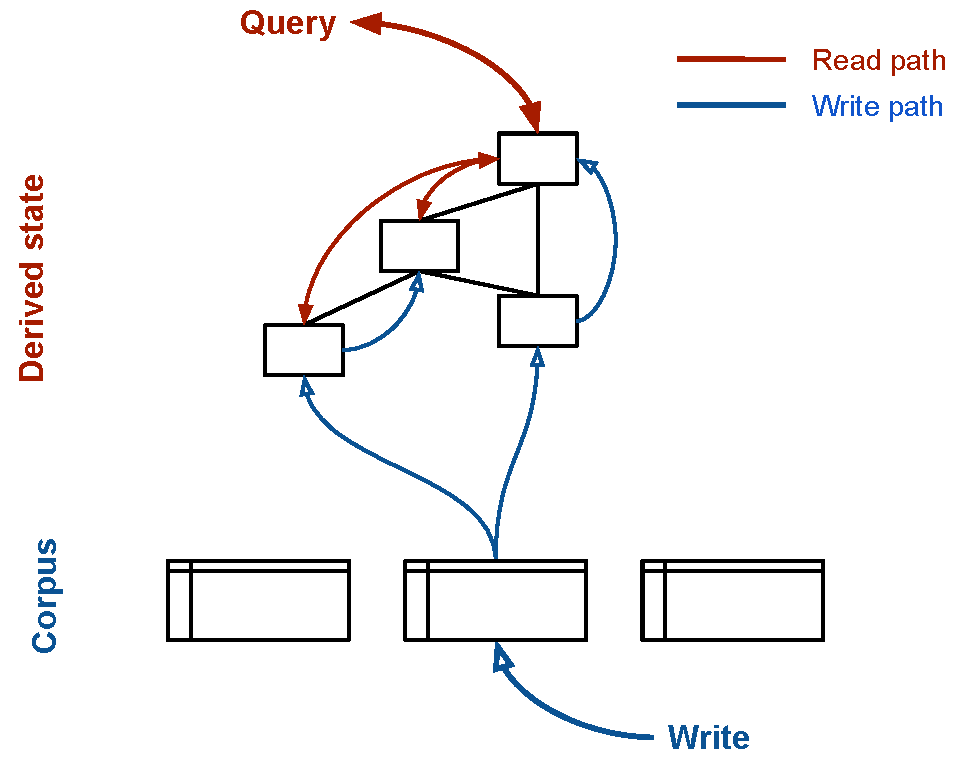
\includegraphics[width=0.5\textwidth]{./figures/design_space/read_write_path.pdf}
  \caption{A conceptual depiction of the derived state's read and write path.}
  \label{fig:design_space_read_write_path}
\end{figure}

\noindent
Figure~\ref{fig:design_space_read_write_path} shows a conceptual depiction of a generic derived state structure's read
and write path.

\textbf{Read path.}
Given a query, the read path consists of sending a message (the query request) from the query source (the client or a query manager component)
to the derived state, performing a query processing computation (for example an index lookup) at the derived state,
and sending a message (the response) back to the query source.
The query processing computation may itself involve additional communication, for example contacting other components of
the query engine in order to request sub-query results.
% For simplicity, we assume here simple predicate queries that do not involve more complex operations such as joins.

\textbf{Write path.}
Given a change to the corpus,
the write path consists of sending a message (the update notification) from the corpus to the derived state,
and the computation required to modify the derived state accordingly.
Similarly, updating the derived state may involve additional communication between components of the derived state.


\subsection{Derived state maintenance schemes}
\label{sec:sync_async_maintenance}

% \todo{MUST HAVE: Figure~\ref{fig:maintenance_schemes} (temporary; borrowed) redo}
% In this section,
% we discuss the design decisions involved in updating derived state according to base data updates.
% We focus on updating a secondary index,
% but the results are analogous for materialized views.

Given the following update to a data item $d$:
\[
d.predominantColor := \#c78f83
\]
updating a secondary index on the $predominantColor$ attribute includes the following steps:
\begin{enumerate}
  \item Insert $d$ to the index entry that corresponds to $predominantColor$ $=$ $\#c78f83$.
  \item Remove $d$ from the index entry that corresponds to the previous value of $d.predominantColor$
  (Depending on the protocol, the system might need to retrieve the previous value of $d.predominantColor$ from the data
  storage tier)
\end{enumerate}

In practice, the derived state subscribes to the change log of the corpus.
If the change log contains the information about the value of $d.predominantColor$ before the change, then step (2) is not
required.

There are different design choices for \textit{when} these steps are performed, relative to the critical
path of the write operation.
We call this design choice, the derived state's \textit{maintenance scheme}.

In \textit{synchronous maintenance}, all maintenance steps are performed in the critical path of the write operation,
typically within the same transaction.
This ensures that derived state is always up-to-date with the corpus,
but increases the write operation's response time.

An alternative approach is to perform some of the maintenance steps \textit{asynchronously}:
deferring them for after the write operation has been acknowledged to the client.
This reduces the overhead to write response time.
However, it also allows derived state to be temporarily \textit{stale}:
For a given write operation, there is a time window in which a data item has been updated,
but the update has not been reflected in the derived state.
As described in Section~\ref{sec:models_freshness},
serving queries from derived state that is stale relative to the corpus may result in query results with false positives
and false negatives.

Amazon's DynamoDB maintains its global secondary indexes asynchronously.
As a result, applications need to ``anticipate and handle situations where a query on a secondary index returns results that are
not up to date'' \cite{dynamodb:async}.

We can reason about derived state maintenance schemes using the framework for derived state's read and write path.
The system can perform tasks in the write path synchronously or asynchronously.
Synchronous write path tasks incur overhead in write operation response time;
Asynchronous ones relax the consistency between corpus and derived state.
As a result, the choice of maintenance scheme involves a trade-off between write response time and query processing effectiveness (\S\ref{sec:requirements}).
The following asynchronous state maintenance schemes have been proposed in the literature:
% \begin{figure}
%   \centering

%   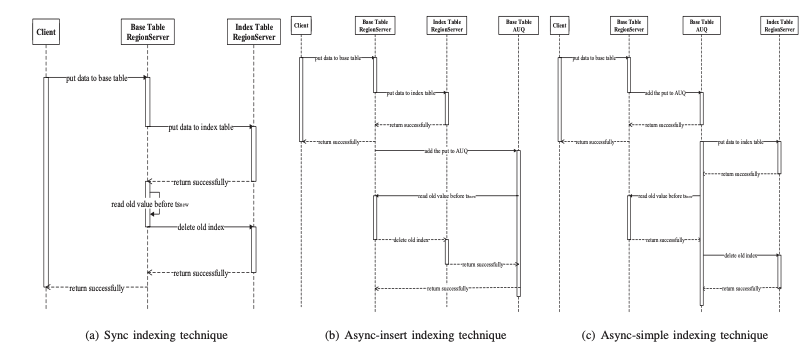
\includegraphics[width=\textwidth]{./figures/design_space/maintenance.png}

%   \caption{Sequence diagram for sync (left), sync-insert (middle), async-simple (right) maintenance}

%   \label{fig:maintenance_schemes}

% \end{figure}

\bigskip
\noindent
\textbf{Sync-insert}

\noindent
One asynchronous maintenance scheme consists of inserting new derived state entries synchronously,
and removing the old state entries asynchronously in the background.
The literature often refers to this scheme as \textit{sync-insert}.

Sync-insert reduces the amount of work in the critical path of write operations,
but it removes stale entries from the derived state asynchronously.
Leaving stale entries in the derived state for a time window means that query results may contain false positives.

The sync-insert scheme is often complemented with a mechanism that,
after reading from the derived state, removes false positives by validating the retrieved results against
the corpus.
This approach trades additional work in the read path, for improved query processing effectiveness.

\bigskip
\noindent
\textbf{Async-simple}

\noindent
In the \textit{async-simple} asynchronous scheme,
a write operation updates the corpus and returns immediately,
deferring the derived state maintenance steps to later.
In practice, async-simple is implemented using an asynchronous update queue:
a write operation is acknowledged as soon as it is logged in the queue;
a background process ingests the queue and updates the derived state.

This scheme incurs minimal overhead to write operations.
However, because it performs all state maintenance tasks asynchronously,
both false positives and negatives are possible.
More specifically, considering an update that changes $d.attributeA$ from $x$ to $y$:
\begin{itemize}
  \item If none of the state maintenance steps have been performed, queries will return as if $x$ is the value of $d.attributeA$
  (false positive and false negative).

  \item If the entry for $d.attributeA$ $=$ $x$ has been removed from the derived state, but the new value has not been
  inserted, $d$ will not appear in query results (false negative).

  \item If the entry for $d.attributeA$ $=$ $y$ has been inserted to the derived state, but the old value has not been
  removed, $d$ will appear in query results for both values (false positive).
\end{itemize}

% Diff-Index \cite{tan:diffindex} has proposed an asynchronous index maintenance scheme that provides sessions guarantees.
% The technique used to achieve this is to track additional state in the client library:
% this state is used to guarantee that any index look-up contains updates to the base data that were made in the same
% session.
% This guarantees the read-your-writes property.

\subsection{Derived state partitioning}
\label{sec:index_partitioning_design_space}

% \todo{MUST HAVE: Figures~\ref{fig:prob1_6_2} and~\ref{fig:prob1_6_1} (temporary; borrowed) redo}

Scaling derived state both in terms of size and and read access requires partitioning it across multiple system nodes.
% The same partitioning schemes can be applied to a materialized view.
% In the rest of this section we refer to secondary indexes.
% The same results apply to Materialized views.
% \todo{results apply to MVs}
In Chapter~\ref{ch:background}, we presented the two main index partitioning schemes.
Briefly:

\begin{itemize}
  \item In \textbf{partitioning by document}, index entries are co-located in the same node as the corresponding
  data items.
  \item In \textbf{partitioning by term}, the index is distributed independently from the corpus.
\end{itemize}

In the partitioning-by-document approach, an index lookup requires a scatter-gather operation:
the system sends a lookup request to every index partition, and then combines the returned results.
An advantage of this approach is that updating the index upon a write to the corpus does not require communication between nodes,
since every data item is, by design, co-located with the index entries it may belong to.

In the partitioning-by-term approach, reading from the index requires contacting only index partitions that hold index entries
relevant to the query.
Updating a term-partitioned index, however, may require communication between nodes,
as index entries may be located on a different node than the data item.

In summary, using the read and write path framework:
Partitioning-by-document guarantees local-only communication on the write path, but requires a large volume of
communication between nodes on the read path (a scatter-gather operation involving all partitions);
Partitioning-by-term involves communication across nodes on the write path (a change to data item may need to be sent to
an index partition on another node),
but requires less communication on the read path in the general case
(index partitions known do not include relevant index entries are not contacted).

% \begin{figure}
%     \centering
%     \begin{minipage}{.5\textwidth}
%         \centering
%         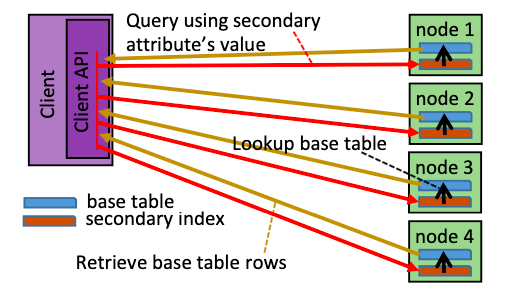
\includegraphics[scale=0.3]{figures/design_space/communication_pattern_document_partitioned.png}
%         \caption{}
%         \label{fig:prob1_6_2}
%     \end{minipage}%
%     \begin{minipage}{0.5\textwidth}
%         \centering
%         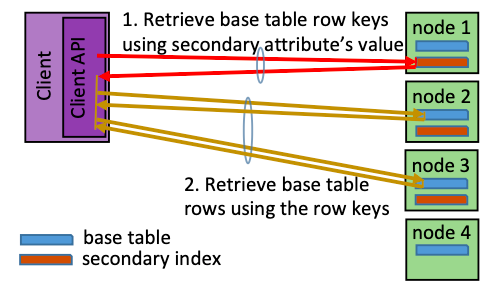
\includegraphics[scale=0.3]{figures/design_space/communication_pattern_term_partitioned.png}
%         \caption{}
%         \label{fig:prob1_6_1}
%     \end{minipage}
% \end{figure}

Guided by this analysis, we can reason about the performance characteristics of the two approaches.

Partitioning-by-document is more suitable at a small scale (small number of nodes),
while partitioning-by-term becomes more suitable as the number of nodes increases,
and has been shown to provide better scalability \cite{kejriwal:slik}.

In addition to the system's architecture scale,
which approach is more suitable depends on a number of different workload characteristics.
D'silva et al. \cite{dsilva:tworings} perform an extensive experimental comparison of the two approaches,
implemented in HBase \cite{hbase:doc}, and show how various workload characteristic affect the index partitioning scheme's performance.

% Key factors that affect index lookup performance are:
% \begin{itemize}

%   % \item The distribution of the values of the indexed attribute:
%   % As the number of data items per index value increases, partitioning-by-document performs better.
%   % This is because the partitioning-by-document performs better when there are
%   % more records to be returned, as index entries are always co-located on the same node as
%   % the index entries.
%   % This is because of the additional round trip required to retrieve the base data items:
%   % as the number of data items per index value increases, a term-partitioned index is likely to have to contact
%   % more and more remote nodes, while  data items are always co-located on the same node as
%   % the index entries.

%   \item Concurrency:
%   As the number of concurrent index lookups increases, partitioning-by-term performs better.
%   This can be attributed to the overhead of the scatter/gather operation used by the document-partitioned index:
%   As the volume of concurrent index lookups increases,
%   the overhead of broadcasting to every node becomes more significant.

%   \item The selectivity of queries:
%   The document-partitioned index outperforms the term-partitioned index as the range size in range queries increases.
%   This is in accordance with the observation that partitioning-by-document is beneficial when there are
%   more records to be returned.

% \end{itemize}

% Additionally, this work assumes synchronous index maintenance, and evaluates the impact of the two approach to write
% operations.
% The document-partitioned index generally outperforms the term-partitioned for writes,
% incurring less overhead to write latency and providing better scalability.


The evaluation results show that:
\begin{itemize}

  \item Partitioning-by-document is more suitable for:
  (1) smaller scale systems with a small number of nodes and light index lookup concurrency,
  (2) workloads with less selective queries that return large result sets,
  (3) skewed data distribution where a large number of data items have the same indexed value,
  or (4) write-intensive workloads.

  \item Partitioning-by-term is more suitable for:
  (1) larger scale systems with a greater number of nodes,
  (2) query-intensive workloads with a large query load,
  (3) workloads consisting of more selective queries with smaller result sets,
  or (4) data with normal distribution of the indexed value.

\end{itemize}

From these results, it is evident that neither of the two approaches is suitable for all needs.
The choice of which approach to use should be guided by factors including the scale of the system,
the properties of the corpus (distribution of indexed values over the data items),
and the characteristics of the workload (query/write ratio, concurrency, query selectivity).

Clearly, the decision of which index partitioning approach to be used needs be taken in a case-by-case basis.
% Database systems should support both index partitioning schemes, and expose the partitioning scheme selection as a
% configuration parameter.
We are not aware of any database system that provides this functionality.
In existing database systems,
the query processing system supports a single in index partitioning scheme (chosen by the database architect) \cite{kejriwal:slik, tan:diffindex, riakv:secondaryindexes, cassandra:secondaryindexing};
every index is partitioned using the same scheme.
In Section~\ref{sec:cs_index_partitioning} we present an approach for making the index partitioning scheme flexible,
and exposing the choice of partitioning scheme as a configuration parameter to the application developer.

\subsection{Derived state placement}
\label{sec:topology_patterns}
% \todo{MUST HAVE: not a good title: should include the term ``placement''}

% \todo{discuss existing approaches for placement of query processing operators across servers for minimizing cross-server communication}

So far in our analysis,
we have considered a case in which corpus, derived state, and clients are placed on the same site,
and therefore, that communication latency among them is not significant.
However, in modern internet-scale services this is often not the case:
Users are typically spread across multiple geographic locations;
Database systems distribute or replicate data across geographically distributed data centers
in order to minimize response time and to improve fault-tolerance.

Long-distance inter- data center network links exhibit latencies in the order of tens to hundreds of milliseconds \cite{pbailis:hats}.
This is an order of magnitude higher than latencies within a data center,
and latencies experienced by users served from a data center close to their geographic location.

In this setting, design choices about 1) the placement of derived state,
2) the communication patterns between corpus and derived state, and 3) the communication patterns between derived state and clients,
determine whether the read and write path computations require communication across data centers.
Performing inter- data center communication in the read or the write path,
incurs significant overheads.
Inter- data center communication on the read path leads to increased query response time.
Inter- data center communication on the write path either increases the delay between a write operation and the corresponding
derived state update (in asynchronous maintenance),
or increases the response time of write operations (in synchronous maintenance).
Additionally, communication across data centers consumes cross-site network resources:
In public cloud pricing models, cross-site data transfer incurs additional monetary cost.
Therefore, in a geo-distributed setting,
these design decisions play a major role in the query processing system's behavior.
% We refer to these design choices as \textit{topology patterns}.

Design choices related to inter- data center communication exacerbate the trade-offs presented in the previous sections,
but also pose additional trade-offs related to the replication of derived state.
In this section, we discuss a number of scenarios that involve geo-distribution and the associated derived state placement approaches.
We will use a secondary index as our running example; however, the analysis also applies to materialized views.

\subsubsection{Geo-replication}
% Cloud-scale database systems rely on geo-distribution to minimize response time and to improve fault-tolerance.
Given a database that is replicated across multiple data centers, we consider the design choices for the architecture
of a query engine that maintains a secondary index.

\begin{figure}[H]
  \centering
  \begin{subfigure}[b]{0.48\textwidth}
    \centering
    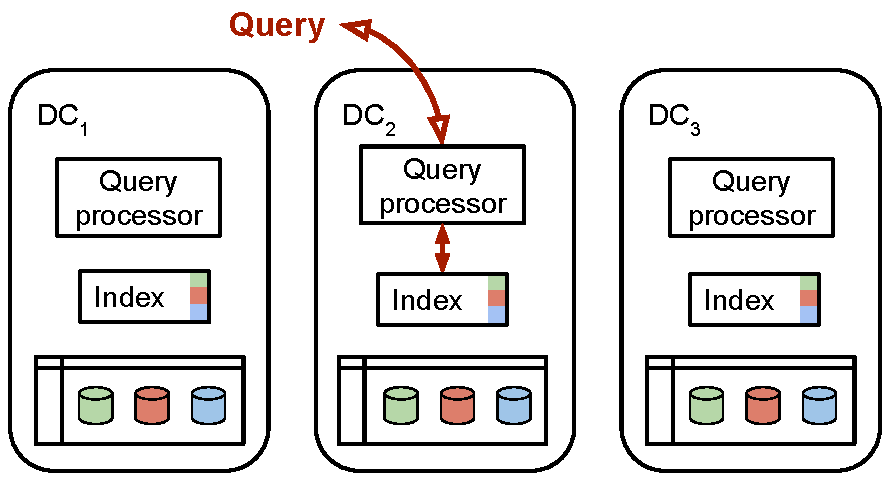
\includegraphics[width=\textwidth]{./figures/design_space/index_full_replication.pdf}
    \caption{}
    \label{fig:index_full_replication}
  \end{subfigure}
  \hfill
  \begin{subfigure}[b]{0.48\textwidth}
    \centering
    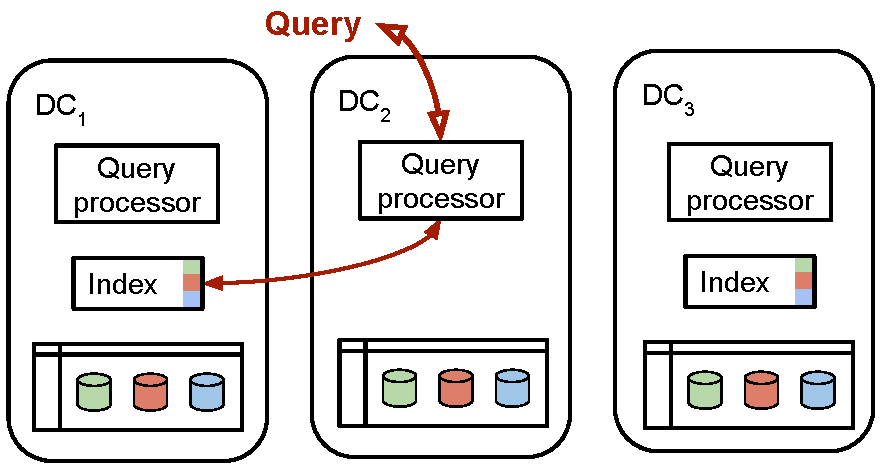
\includegraphics[width=\textwidth]{./figures/design_space/index_partial_replication.pdf}
    \caption{}
    \label{fig:index_partial_replication}
  \end{subfigure}
  \caption{Index placement schemes over a geo-replicated corpus.}
  \label{fig:index_placement_geo_replication}
\end{figure}

One approach is to maintain a replica of the index on each data center (Figure~\ref{fig:index_full_replication}).
With this approach, both the read and write path involve only intra- data center communication:
Queries can be served from the index at the closest date center, without requiring communication with
remote data centers.
Index maintenance is also local, since the entire corpus is present on each data center.
The downside of this approach is the additional memory and storage resources required for maintaining index replicas.

An alternative approach is to place index replicas on a subset of the data centers.
This reduces the storage overhead, but means that a query sent to a data center without an index
either needs to be forwarded to another data center (Figure~\ref{fig:index_partial_replication}), or be processed without using the index,
both of which result in slower query processing.
This approach is more suitable for cases in which some data centers receive more queries than others.
Moreover, this approach can be supplemented with the use of caches in data centers without index replicas.

% This architecture poses a design choice which
% from an impossibility property, known as the [60].
% In addition, strongly-consistent designs are susceptible to downtimes due to network partitions. In a highly-available design, replicas synchronize in the background, out of the critical path of write operations. This ensures low latency and availability under network par- titions, as each replica serves write operations locally. Nevertheless, this allows replicas to accept concurrent conflicting updates and temporary diverge.

\subsubsection{Geo-partitioning}
A different geo-distribution strategy is geo-partitioning.
In geo-partitioning, data is partitioned across data centers, and partitions are placed on data centers according to
their access patterns.
As a result, read and write access to data that belongs to a local partition is fast.
CockroachDB for example, allows developers to partition data across data centers with row granularity
\cite{cockroachdb:geopartitioning}.

\begin{figure}[H]
  \centering
  \begin{subfigure}[b]{0.48\textwidth}
    \centering
    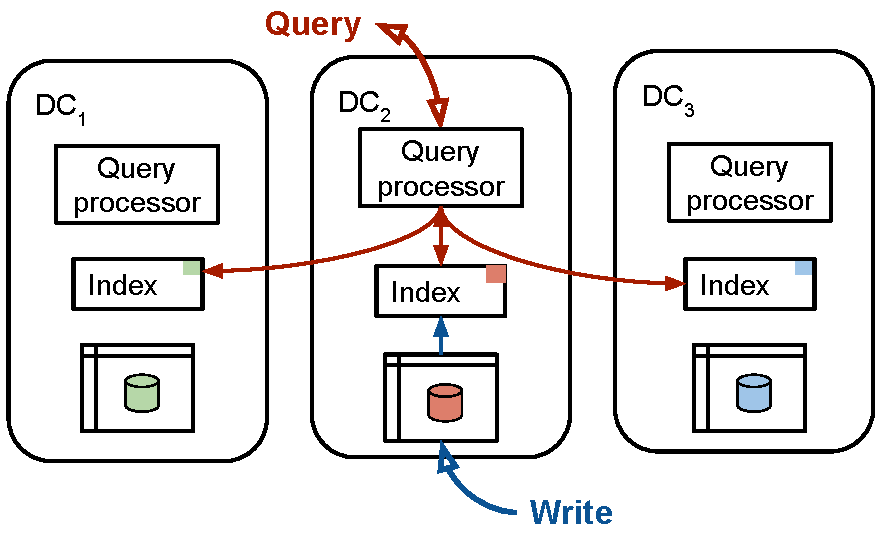
\includegraphics[width=\textwidth]{./figures/design_space/geo_paritioning_local_index.pdf}
    \caption{}
    \label{fig:geo_paritioning_local_index}
  \end{subfigure}
  \hfill
  \begin{subfigure}[b]{0.48\textwidth}
    \centering
    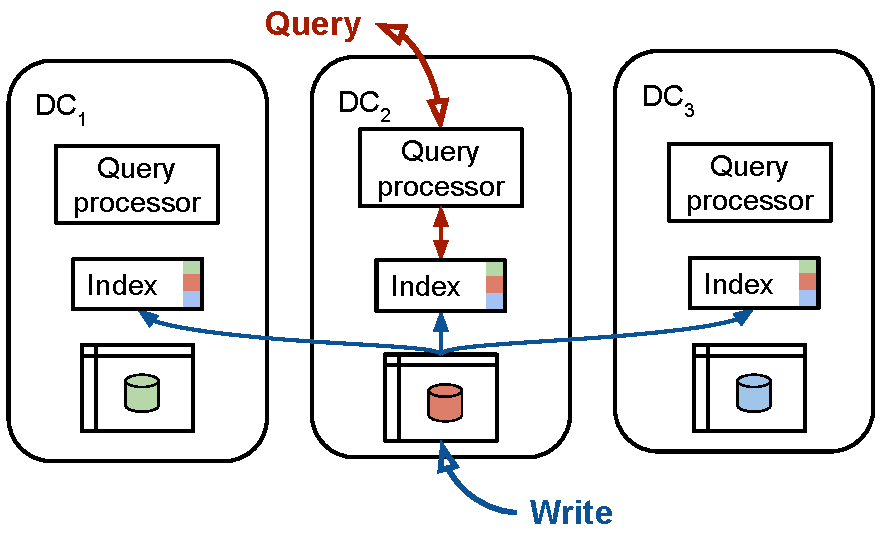
\includegraphics[width=\textwidth]{./figures/design_space/geo_paritioning_global_indexes.pdf}
    \caption{}
    \label{fig:geo_paritioning_global_indexes}
  \end{subfigure}
  \caption{Index placement schemes over a geo-partitioned corpus.}
  \label{fig:index_placement_geo_partitioning}
\end{figure}

One approach for maintaining a secondary index over geo-partitioned data is to use the partitioning-by-document scheme:
each data center maintains a secondary index covering the local data items (Figure~\ref{fig:geo_paritioning_local_index}).
This approach has the same implications as document-based partitioning:
the write path requires only intra- data center communication, since the index is co-located with the corresponding data items;
the read path needs to contact the index partition on every data center, and gather the results.

A different approach is to maintain a global secondary index on each data center (Figure~\ref{fig:geo_paritioning_global_indexes}).
In that case, the index lookups (read path) can always be served locally.
However, each change to the corpus needs to be propagated to all data centers (write path).
The downside of this approach is that it significantly increases the memory and storage cost required for maintaining the
index replicas.

\subsubsection{Multi-cloud and Query federation}
More recently, the concept of multi-cloud data storage has emerged.
Organizations spread their data across private data centers and public cloud services in order to reduce costs and
ensure fault-tolerance.
Moreover, they distribute data across multiple cloud providers in order to avoid dependence on a single
cloud provider, take advantage of diverse storage and computing services, and improve reliability.

The advent of data distributed across multiple independent storage systems has created the need for unified access and
federated search across platforms.
The problem of federated query processing can be viewed as a generalization of the geo-partitioning case:
the corpus at each platform can be seen as a partition of the logical global corpus.
For simplicity, we assume that a multi-cloud platform consists of multiple, independent instances of a common database
system.
Under there assumptions, the same design decisions and trade-offs as in the case of geo-partitioning apply to query
federation across multiple clouds.
The same observations can be generalized to heterogeneous systems composed of different database system.
However, federated query processing includes additional challenges linked to the heterogeneous data models of these
systems.

From this analysis, it becomes clear that derived state placement and its communication patterns with the corpus and
clients play a major role in the performance of geo-distributed query processing.

\section{Conclusion}

% \todo{GOOD TO HAVE: we need a vizualization \\ multi-dimensional table? decision tree? something else?}

\begin{itemize}
  \item The use of derived state to speed-up query processing moves query processing work from the read path to the write
  path, while also incurring memory and storage overhead.
  Moreover, different derived state schemes (indexes, materialized views, caching) entail different amount of work
  on the read and write path.

  \item The choice of derived state maintenance scheme controls the impact of work on the write path:
  Synchronous maintenance keeps derived state up-to-date with the corpus,
  but incurs overhead to the latency of write operations.
  On the other hand, asynchronous maintenance schemes move some of the work on the write path in the background.
  This reduces the overhead to write operations, but also means that derived state is not always up-to-date with the base
  data.
  Because serving queries from derived state that is stale relative to the corpus may introduce false positives and
  false negatives,
  design decisions on derived state maintenance pose a trade-off between the overhead to write operations
  and the relevance of query results.

  \item The derived state partitioning scheme determines the communication patterns between corpus and derived state
  on the write path, and between derived state and client on the read path.
  More specifically, partitioning-by-document ensures that no cross-node communication is needed on the write path,
  but requires a scatter/gather operation across all state partitions on the read path.
  Partitioning-by-term requires cross-node communication on the write path but reduces the number of state partitions
  that need to participate on the read path.
  Therefore, the choice of partitioning scheme poses a trade-off in the type (intra-node or cross-node) and volume
  of communication on the read versus the write path.

  \item When corpus and clients are distributed across different geographic locations,
  derived state placement affects communication latency (intra versus inter data center communication)
  between derived state and corpus and between derived state and clients.
  This creates a number of trade-offs, that result from the basic trade-off of requiring intra data center communication
  on the read versus the write path.
  These trade-offs include:
  \begin{itemize}
    \item Low latency on the read path versus increased latency on the write path in the case of synchronous maintenance,
    or decreased freshness in the case of asynchronous maintenance.
    \item Low latency on the read path versus increased resource utilization for maintaining derived state replicas,
    and increased volume of write path communication.
    \item Low data transfer cost on the read path versus on the write path.
  \end{itemize}

\end{itemize}